Para comparar os cinco métodos utilizados, testamos quatro funções com o objetivo de descobrir os pontos fracos e fortes de cada método. Para facilitar essa comparação, analisaremos os resultados obtidos por cada método no programa criado.

\begin{itemize}
	\item Para o primeiro caso, foi utilizada a função $ \mathbf{f_1(x,y) = x^2 + y^2} $ com ponto inicial em (2,2)
\end{itemize}


\begin{figure}[H]
	\centering
	\begin{minipage}{.5\textwidth}
		\centering
		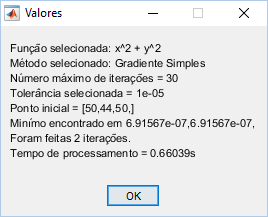
\includegraphics[width=7cm]{../stegrades/f1_resultados.PNG}
		\caption{Resultados de $ f_1 $ (Gradiente)}
		\label{fig:resultados_grad_f1}
	\end{minipage}%
	\begin{minipage}{.5\textwidth}
		\centering
		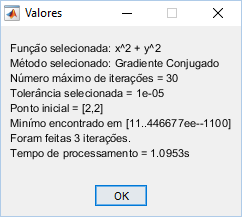
\includegraphics[width=6.5cm]{../gradiente_conjugado/f1_resultados.PNG}
		\caption{Resultados de $ f_1 $ (Gradiente Conjugado)}
		\label{fig:resultados_grad_conj_f1}
	\end{minipage}
\end{figure}

\begin{figure}[H]
	\centering
	\begin{minipage}{.5\textwidth}
		\centering
		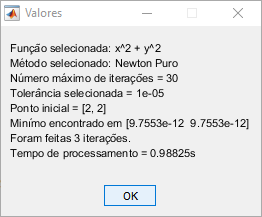
\includegraphics[width=7cm]{../newton/f1_resultados.PNG}
		\caption{Resultados de $ f_1 $ (Newton)}
		\label{fig:resultados_newton_f1}
	\end{minipage}%
	\begin{minipage}{.5\textwidth}
		\centering
		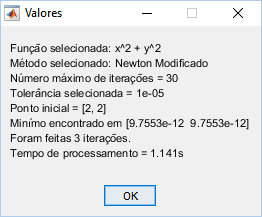
\includegraphics[width=7cm]{../newton_mod/f1_resultados.PNG}
		\caption{Resultados de $ f_1 $ (Newton Modificado)}
		\label{fig:resultados_newton_mod_f1}
	\end{minipage}
\end{figure}

\begin{figure}[H]
	\begin{center}
		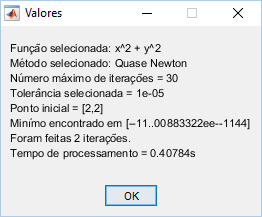
\includegraphics[width=7cm]{../quase_newton/f1_resultados.PNG}   
		\caption{Resultados de $ f_1 $ (Quase Newton)}
		\label{fig:resultados_quase_newton_f1}
	\end{center}
\end{figure}

A função $ \mathbf{f_1(x,y)} $ foi utilizada como controle para os outros testes, por ser uma função simples, e o seu mínimo é facilmente encontrado por todos os métodos, porém alguns se mostraram mais rápidos que outros. O método de Quase Newton se mostrou o mais rápido, além de convergir com apenas duas iterações.

\begin{itemize}
	\item No segundo caso, usamos a função $ \mathbf{f_2(x,y) = -e^{-x^2 -y^2}} $ com ponto inicial em (3,2)
\end{itemize}

\begin{figure}[H]
	\centering
	\begin{minipage}{.5\textwidth}
		\centering
		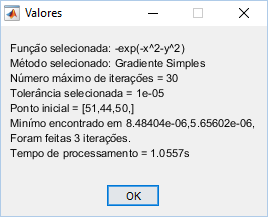
\includegraphics[width=7cm]{../stegrades/f2_resultados.PNG}
		\caption{Resultados de $ f_2 $ (Gradiente)}
		\label{fig:resultados_grad_f2}
	\end{minipage}%
	\begin{minipage}{.5\textwidth}
		\centering
		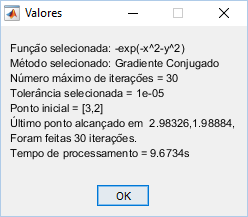
\includegraphics[width=7cm]{../gradiente_conjugado/f2_resultados.PNG}
		\caption{Resultados de $ f_2 $ (Gradiente Conjugado)}
		\label{fig:resultados_grad_conj_f2}
	\end{minipage}
\end{figure}

\begin{figure}[H]
	\centering
	\begin{minipage}{.5\textwidth}
		\centering
		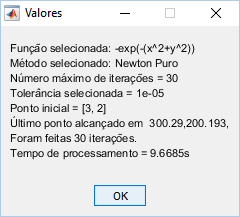
\includegraphics[width=7cm]{../newton/f2_resultados.PNG}
		\caption{Resultados de $ f_2 $ (Newton)}
		\label{fig:resultados_newton_f2}
	\end{minipage}%
	\begin{minipage}{.5\textwidth}
		\centering
		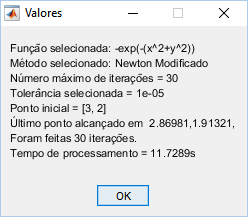
\includegraphics[width=7cm]{../newton_mod/f2_resultados.PNG}
		\caption{Resultados de $ f_2 $ (Newton Modificado)}
		\label{fig:resultados_newton_mod_f2}
	\end{minipage}
\end{figure}

\begin{figure}[H]
	\begin{center}
		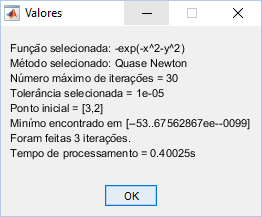
\includegraphics[width=7cm]{../quase_newton/f2_resultados.PNG}   
		\caption{Resultados de $ f_2 $ (Quase Newton)}
		\label{fig:resultados_quase_newton_f2}
	\end{center}
\end{figure}

Por ser uma função com uma descida repentina e ter sido usado um ponto inicial longe do mínimo, os métodos de Newton não funcionam muito bem no geral para a função $ \mathbf{f_2(x,y)} $, já que não é possível criar uma aproximação quadrática para a função escolhida. Por isso, os métodos de Newton e de Newton Modificado fizeram todas as iterações pedidas e não conseguiram alcançar o mínimo. Podemos ver que as melhorias do método de Quase Newton fizeram com que esse método contornasse o problema do método de Newton puro, achando o mínimo da função. O método do Gradiente Conjugado não conseguiu encontrar o mínimo mesmo depois de todas as iterações.


\begin{itemize}
	\item Como terceiro teste, usamos a função $ \mathbf{f_3(x,y) = cos(\frac{xy}{5})+sin(\frac{xy}{5})} $ com ponto inicial em (1,3)
\end{itemize}


\begin{figure}[H]
	\centering
	\begin{minipage}{.5\textwidth}
		\centering
		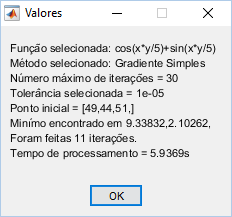
\includegraphics[width=6.5cm]{../stegrades/f3_resultados.PNG}
		\caption{Resultados de $ f_3 $ (Gradiente)}
		\label{fig:resultados_grad_f3}
	\end{minipage}%
	\begin{minipage}{.5\textwidth}
		\centering
		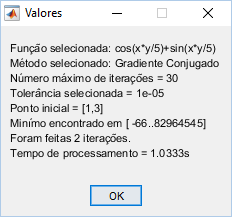
\includegraphics[width=6.5cm]{../gradiente_conjugado/f3_resultados.PNG}
		\caption{Resultados de $ f_3 $ (Gradiente Conjugado)}
		\label{fig:resultados_grad_conj_f3}
	\end{minipage}
\end{figure}

\begin{figure}[H]
	\centering
	\begin{minipage}{.5\textwidth}
		\centering
		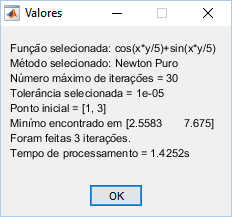
\includegraphics[width=6.5cm]{../newton/f3_resultados.PNG}
		\caption{Resultados de $ f_3 $ (Newton)}
		\label{fig:resultados_newton_f3}
	\end{minipage}%
	\begin{minipage}{.5\textwidth}
		\centering
		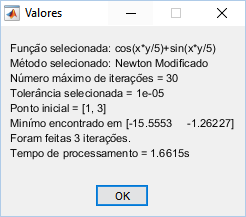
\includegraphics[width=7cm]{../newton_mod/f3_resultados.PNG}
		\caption{Resultados de $ f_3 $ (Newton Modificado)}
		\label{fig:resultados_newton_mod_f3}
	\end{minipage}
\end{figure}

\begin{figure}[H]
	\begin{center}
		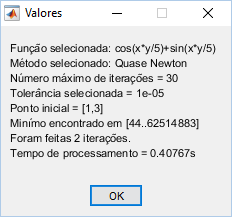
\includegraphics[width=6cm]{../quase_newton/f3_resultados.PNG}   
		\caption{Resultados de $ f_3 $ (Quase Newton)}
		\label{fig:resultados_quase_newton_f3}
	\end{center}
\end{figure}

Podemos ver que, para a função $ \mathbf{f_3(x,y)} $, os métodos de Newton, Newton Modificado e Quase Newton funcionaram bem, convergindo com poucas iterações e rapidamente. O método do Gradiente não funcionou tão bem, por ter sido aplicado em uma função com muitas ondulações. As alterações implementadas no método do Gradiente Conjugado fizeram com que esse método conseguisse encontrar o mínimo com relativa facilidade, em apenas duas iterações.


\begin{itemize}
	\item Para a última comparação, foi testada a função $ \mathbf{f_4(x,y) = |x+y|} $ com ponto inicial em (1,1)
\end{itemize}


\begin{figure}[H]
	\centering
	\begin{minipage}{.5\textwidth}
		\centering
		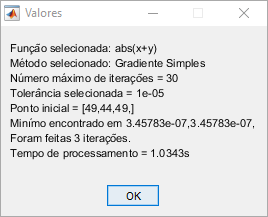
\includegraphics[width=7cm]{../stegrades/f4_resultados.PNG}
		\caption{Resultados de $ f_4 $ (Gradiente)}
		\label{fig:resultados_grad_f4}
	\end{minipage}%
	\begin{minipage}{.5\textwidth}
		\centering
		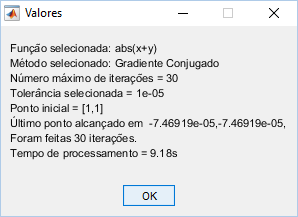
\includegraphics[width=7.5cm]{../gradiente_conjugado/f4_resultados.PNG}
		\caption{Resultados de $ f_4 $ (Gradiente Conjugado)}
		\label{fig:resultados_grad_conj_f4}
	\end{minipage}
\end{figure}

\begin{figure}[H]
	\centering
	\begin{minipage}{.5\textwidth}
		\centering
		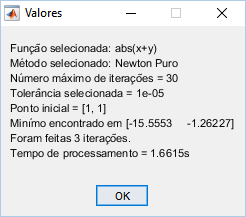
\includegraphics[width=7cm]{../newton/f4_resultados.PNG}
		\caption{Resultados de $ f_4 $ (Newton)}
		\label{fig:resultados_newton_f4}
	\end{minipage}%
	\begin{minipage}{.5\textwidth}
		\centering
		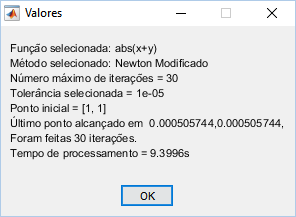
\includegraphics[width=7.5cm]{../newton_mod/f4_resultados.PNG}
		\caption{Resultados de $ f_4 $ (Newton Modificado)}
		\label{fig:resultados_newton_mod_f4}
	\end{minipage}
\end{figure}

\begin{figure}[H]
	\begin{center}
		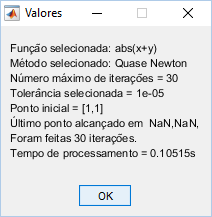
\includegraphics[width=7cm]{../quase_newton/f4_resultados.PNG}   
		\caption{Resultados de $ f_4 $ (Quase Newton)}
		\label{fig:resultados_quase_newton_f4}
	\end{center}
\end{figure}

Alguns métodos tiveram dificuldades para encontrar o mínimo da função $ \mathbf{f_4(x,y)} $, devido ao fato de que essa função possui um bico no seu mínimo, o que dificulta a ação dos métodos de Newton, por isso, o método de Quase Newton não conseguiu encontrar um mínimo, e o método de Newton Modificado fez todas as iterações pedidas, demorando quase 10 segundos para encontrar um valor. O método do Gradiente conseguiu encontrar facilmente o mínimo, em apenas 3 iterações, enquanto que o método do Gradiente Modificado teve que usar o número máximo de iterações para encontrar um valor.

Podemos então concluir que não existe um método absoluto para localização de mínimos de funções vetoriais, mas podemos classificar alguns métodos em seções. Os métodos de Newton costumam funcionar melhor para funções que admitem boas aproximações quadráticas, enquanto que os métodos do tipo Gradiente não costumam funcionar muito bem se a função objetivo oscila muito rapidamente.